
\documentclass[a4paper,UKenglish,cleveref, autoref, thm-restate]{lipics-v2021}
%This is a template for producing LIPIcs articles. 
%See lipics-v2021-authors-guidelines.pdf for further information.
%for A4 paper format use option "a4paper", for US-letter use option "letterpaper"
%for british hyphenation rules use option "UKenglish", for american hyphenation rules use option "USenglish"
%for section-numbered lemmas etc., use "numberwithinsect"
%for enabling cleveref support, use "cleveref"
%for enabling autoref support, use "autoref"
%for anonymousing the authors (e.g. for double-blind review), add "anonymous"
%for enabling thm-restate support, use "thm-restate"
%for enabling a two-column layout for the author/affilation part (only applicable for > 6 authors), use "authorcolumns"
%for producing a PDF according the PDF/A standard, add "pdfa"

%\pdfoutput=1 %uncomment to ensure pdflatex processing (mandatatory e.g. to submit to arXiv)
%\hideLIPIcs  %uncomment to remove references to LIPIcs series (logo, DOI, ...), e.g. when preparing a pre-final version to be uploaded to arXiv or another public repository

%\graphicspath{{./graphics/}}%helpful if your graphic files are in another directory

\bibliographystyle{plainurl}% the mandatory bibstyle

\title{A Verified Implementation of B$^+$-Trees in Isabelle/HOL} %TODO Please add

%\titlerunning{Dummy short title} %TODO optional, please use if title is longer than one line

\author{Niels Mündler}{Department of Computer Science, ETH Zurich, Switzerland}{n.muendler@tum.de}{https://orcid.org/0000-0003-3851-2557}{}%TODO mandatory, please use full name; only 1 author per \author macro; first two parameters are mandatory, other parameters can be empty. Please provide at least the name of the affiliation and the country. The full address is optional. Use additional curly braces to indicate the correct name splitting when the last name consists of multiple name parts.

\author{Tobias Nipkow}{Department of Informatics, Technical University of Munich, Germany}{nipkow@in.tum.de}{https://orcid.org/0000-0003-0730-515X}{}

\author{Peter Lammich}{Department of Computer Science, The University of Manchester, Great-Britain}{lammich@in.tum.de}{https://orcid.org/0000-0003-3576-0504}{}

\authorrunning{N. Mündler, T. Nipkow and P. Lammich} %TODO mandatory. First: Use abbreviated first/middle names. Second (only in severe cases): Use first author plus 'et al.'

\Copyright{Niels Mündler} %TODO mandatory, please use full first names. LIPIcs license is "CC-BY";  http://creativecommons.org/licenses/by/3.0/

\begin{CCSXML}
    <ccs2012>
       <concept>
           <concept_id>10003752.10003790.10011742</concept_id>
           <concept_desc>Theory of computation~Separation logic</concept_desc>
           <concept_significance>500</concept_significance>
           </concept>
     </ccs2012>
\end{CCSXML}
    
\ccsdesc[500]{Theory of computation~Separation logic}
%TODO mandatory: Please choose ACM 2012 classifications from https://dl.acm.org/ccs/ccs_flat.cfm 

\keywords{Separation Logic, Verification, Refinement} %TODO mandatory; please add comma-separated list of keywords

\category{} %optional, e.g. invited paper

\relatedversion{} %optional, e.g. full version hosted on arXiv, HAL, or other respository/website
%\relatedversiondetails[linktext={opt. text shown instead of the URL}, cite=DBLP:books/mk/GrayR93]{Classification (e.g. Full Version, Extended Version, Previous Version}{URL to related version} %linktext and cite are optional

%\supplement{}%optional, e.g. related research data, source code, ... hosted on a repository like zenodo, figshare, GitHub, ...
%\supplementdetails[linktext={opt. text shown instead of the URL}, cite=DBLP:books/mk/GrayR93, subcategory={Description, Subcategory}, swhid={Software Heritage Identifier}]{General Classification (e.g. Software, Dataset, Model, ...)}{URL to related version} %linktext, cite, and subcategory are optional

%\funding{(Optional) general funding statement \dots}%optional, to capture a funding statement, which applies to all authors. Please enter author specific funding statements as fifth argument of the \author macro.

\acknowledgements{I want to thank \dots}%optional

%\nolinenumbers %uncomment to disable line numbering



%Editor-only macros:: begin (do not touch as author)%%%%%%%%%%%%%%%%%%%%%%%%%%%%%%%%%%
\EventEditors{John Q. Open and Joan R. Access}
\EventNoEds{2}
\EventLongTitle{42nd Conference on Very Important Topics (CVIT 2016)}
\EventShortTitle{CVIT 2016}
\EventAcronym{CVIT}
\EventYear{2016}
\EventDate{December 24--27, 2016}
\EventLocation{Little Whinging, United Kingdom}
\EventLogo{}
\SeriesVolume{42}
\ArticleNo{23}
%%%%%%%%%%%%%%%%%%%%%%%%%%%%%%%%%%%%%%%%%%%%%%%%%%%%%%

\newcommand{\btree}{B$^+$-Tree}
\newcommand{\btrees}{B$^+$-Trees}

\begin{document}

\maketitle

%TODO mandatory: add short abstract of the document
\begin{abstract}
    The abstract will surely become longer at some point.
\end{abstract}

\section{Introduction}
\label{sec:introduction}

This will be the introduction. There will be more text.

\subsection{Related Work}
\label{sec:related_work}

Ernst verified a simplified version of \btrees that does
not have links between leaf nodes.

Malecha already built and verified \btrees \cite{}.
In their approach, they chose an intermediate layer of a functional
data structure that explicitely stores pointers to their heap embedded
correspondence.

\subsection{Contributions}
\label{sec:contributions}

We provide an alternative approach to verifying \btree implementations,
by fully separating the functional and imperative layers.
This allows for complex relationships to be validated on a purely
functional level, while on the imperative level
only refinement of the abstract operations needs to be shown.
The approach allowed us to supplement the implementation
with an efficient binary search on the node level
and eventually provide an efficient range query iterator
on top of a list element iterator.


\section{\btrees\ and Approach}
\label{sec:approach}

B-trees were first proposed by Bayer in \cite{DBLP:journals/acta/BayerM72},
as a data-structure to efficiently retrieve and manipulate
indexed data stored on storage devices with slow memory access.
They are $n$-ary balanced search trees.
They may be specified as implementing a set interface,
where the indices form the actual content of the set,
the specification that serves as basis in this work.

A commonly implemented variation is the \btree, where the inner nodes
only contain separators to guide the recursive navigation through the tree.
In \btrees, all data is stored in the leaves \cite{DBLP:journals/csur/Comer79}.
Further the leaves are usually implemented so as to contain pointers
to the next leaf in order, allowing for efficient iterators and range queries.

\begin{figure}
    % TODO update figure 
    \centering
    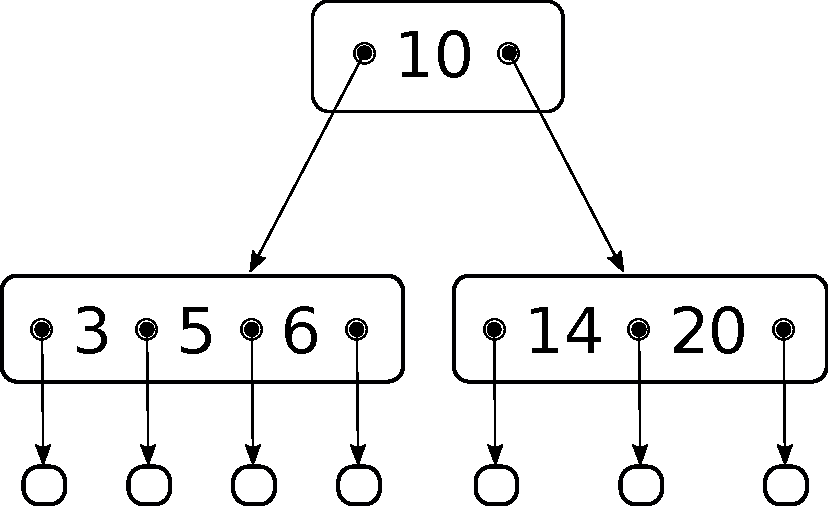
\includegraphics[width=0.5\linewidth]{figures/btree-basic-nopair.pdf}
    \caption[A small example B-Tree]{A small balanced, sorted B-tree of order $2$ and
    height $2$ containing $3$ nodes and $6$ elements.
    In subsequent depictions, leafs will be depicted
    by empty circles.}
    \label{fig:btree-basic-nopair}
\end{figure}


\subsection{Definitions}
\label{sec:data_structure_defs}

Every node contains a list of \textit{keys} (also \textit{separators}, and \textit{subtrees} (\textit{children}),
that represent further \btree nodes.
The separators and subtrees may be considered interleaved within a node,
such that we can speak of a subtree to the left of a separator and
a subtree to the right of a separator,
where for a separator at index $i$ we mean the subtree in the respective
subtree list at index $i$ and $i+1$ respectively.
Note that this already implies that the list of subtrees is one
longer than the list of separators - we refer to the last subtree
as the \textit{last} or \textit{dangling} subtree.
The leafs contain lists of \textit{values}.
A \btree with above structure must fulfill the three properties
\textit{balancedness}, \textit{order} and \textit{sortedness}.

\textbf{Balancedness} requires
that each path from the root to any leaf has the same length $h$.
In other words, the height of all trees in one level of the tree must be equal,
where the height is the maximum path length to any leaf.

Further the keys and values must be \textbf{sorted} within the tree which means that all keys stored
in the subtree to the left of a separator are smaller than the value of the separator
and all indices in the subtree to the right are greater.
Moreover, all values in the subtree to the left of a key must be smaller or equal
to the key and all values in the subtree to the right must be greater.\footnote{
    The exact direction of the part that may contain equal element is a design choice.
}
Further all keys within a node should maintain a sorted order,
as well as all the values within a leaf.

In general terms, the property of \textbf{order} ensures a certain minimum and maximum
number of subtrees for each node.
However, as pointed out by Folk and Zoellick \cite{DBLP:books/daglib/0095349_mod},
the property is defined differently in the literature.
For the purpose of this work, the original definition by Bayer
was chosen as most suitable.
A \btree is of order $k$, if each internal node has at least $k+1$
subtrees and at most $2k+1$.
The root is allowed to have a minimum of 2 and a maximum of $2k+1$ subtrees.

Note that the B-tree definition is only meaningful for positive $k$.
For the case that $k$ is equal to 0,
all elements of the tree would have exactly one subtree
and no internal elements.
For the root node this even leads to a contradictory state:
It is required to contain at least 1 element or 2 subtrees.
However as it should not have more than $2k+1 = 1$ elements,
this constraint can not be satisfied.
Requiring positive $k$ is consistent with the definitions
in the consulted literature \cite{DBLP:journals/acta/BayerM72,DBLP:journals/csur/Comer79,DBLP:books/daglib/0023376}.

\section{Functional \btrees}
\label{sec:functional}

The general goal of the verification is to express
all operations on an abstract level first.
We introduce a generic split function that does node-internal search
for us and provide operations on the whole tree based on them.

\subsection{Set operations}
\label{sec:functional_set}

The most important operations on \btrees are point querys and insertion.
There is a canon on their implementation which we followed in our approach.
Deletion is less commonly implemented and even less verified,
however we provide an a functional definition of a correct deletion operation.

In order to verify these operations it was useful to further
abstract away structures of the tree.
Following Nipkows approach, we could ignore the internal structure of the tree
and provide proofs for the sortedness of the leaf elements purely
based on their respective refinement of sorted lists.
The internal structure of the trees, the navigation separators however,
cannot be abstracted away and require explicit proofs.

\subsection{Range operations}
\label{sec:functional_range}

On the functional level, the forwarding leaf pointers in each leaf
are not present, as this would require aliasing.
Therefore, iterators merely compute the concatenation
of all leaf contents in the trivial manner.
Range iterators then concatenate the correct parts of the
abstract tree.
Only when refining the operations, we will make use of the leaf pointers
to obtain an efficient implementation.


\section{Imperative \btrees}
\label{sec:imperative}

\subsection{Set operations}
\label{sec:imperative_set}

The refinement of set operations is relatively straightforward and
follows in large parts the procedure in my BSCTHesis.
One additional challenge here is to prove the correct initialization
and modification of pointers in the leaves,
as this cannot be proven on the abstract level, where these pointers
have no correspondence.

\subsection{Iterators}
\label{sec:imperative_iter}

In order to be able to iterate over the leafs
a statement on the heap has to be made that relates
a leaf and all leafs in the linked list from there
to a tree rooted in some node.
For this purpose we follow the approach of malecha
to split the tree assertion into an equivalent assertion
on the inner nodes as well as only the concatenated leaf nodes.
In order to make use of the benefits of separation logic,
it is important that these statements only regard separated parts of the heap.

At this point a subtlety of the abstract refinement approach surfaces.
If we only have a statement about some pointers refining some abstract inner nodes
and a statement about some pointers refining some abstract leaf nodes - 
how can we guarantee that these pointers can be glued back together to form the
full abstract tree?

The point is, that we have a situation of aliasing now,
that is in general not well handled by separation logic.
However, we only need the content of one of the aliases, which again is fine
regarding separation logic.
The other statement then simply expresses "the pointer is the same as in the other statement"
which is not an overlapping statement regarding the heap.
Therefore we need to make the sharing here explicit,
obtaining the exact list of pointers in the imperative implementation
and pull them into the refinement relationship.
A nice fact is that we can always obtain this list even from the
refinement relationship that does not have it explicit,
and we can even ignore it again once we wrapped up the whole
iterator assertion into one definition.
To the user, this explicit sharing will hence never surface,
the user only interacts with the tree root pointer and the abstract tree.

\subsection{Range operations}
\label{sec:imperative_range}

One interesting note on the range iterators is, that a
straightforward proof of the correctness of the exact range iterator
failed at the attempt to recursively make a statement on
the leaf element iterators on the subtree.
A workaround is to just make a statement about the split tree first,
and later obtain the iterator only from manipulating the obtained leaf node.
This lead to the functional level being extended by two functions,
one that obtained the correct leaf node for the range iteration
and another one that manipulated the leaf node to obtain
the correct element-level iterator on all values.
On a second attempt, these two functions could then be imperatively
refined and verified.
Their concatenation then yields the intended result at no extra cost.

\subsection{Binary internal search}
\label{sec:imperative_split}

Due to the high abstraction of the proofs,
we can now provide different node internal search algorithms,
as long as they guarantee the required properties of the split function.
To this end we provide a linear search algorithm
and a binary search, the latter being commonly used in real world applications.

\section{Comparison and Conclusion}
\label{sec:conclusion}

We were able to define and verify a number of efficient operations
on imperative \btrees.
Namely we provide the basics with point and insertion querys.
Further we provide an efficient iterator on the leafs
and even give a range operation for a lower bound that
can be trivially extended to support an upper bound.
All operations are conducted on a \btree with linked leafs,
and conduct binary search within each node.

\end{document}
